\documentclass{beamer}
\usetheme{Madrid}


% Define neutral and accent colors
\definecolor{LightGray}{RGB}{245,245,245}
\definecolor{DarkGray}{RGB}{105,105,105}
\definecolor{AccentColor}{RGB}{0,51,153}  % Demokritos Blue as an accent

% Apply the colors
\setbeamercolor{background canvas}{bg=white}
\setbeamercolor{title}{fg=DarkGray, bg=LightGray}
\setbeamercolor{frametitle}{fg=DarkGray, bg=LightGray}
\setbeamercolor{structure}{fg=AccentColor}
\setbeamercolor{item projected}{bg=AccentColor}

\usepackage{hyperref}
\hypersetup{
    colorlinks=true,
    linkcolor=blue,
    urlcolor=cyan,
}
\usepackage{listings}
\lstset{
  basicstyle=\ttfamily\footnotesize,
  breaklines=true,
  frame=single
}


\title{Small-Object Detection in Remote Sensing Images and Video}
\author{Stamatios Orfanos}
\institute{University of Piraeus \hspace*{1cm} NCSR Demokritos}
\date{\today}
\titlegraphic{
\includegraphics[width=4.5cm]{Figures/University-of-Piraeus-logo-350x250.png}\hspace*{1cm}
\includegraphics[width=2cm]{Figures/demokritos-logo.png}}

\begin{document}

\begin{frame}
  \titlepage
\end{frame}

\begin{frame}
  \frametitle{Table of Contents}
  \tableofcontents
\end{frame}

\section{Introduction}
\begin{frame}[t]
  \frametitle{Introduction}
  Remote sensing imaging is a process used to gather information about objects or areas from a distance, typically using aircraft or satellites.
  Remote sensing imaging has applications across a broad spectrum of fields.
  
  \begin{columns}[T]
    \begin{column}{.4\textwidth}
      \begin{itemize}
        \item Environmental monitoring  
        \item Agriculture monitoring    
        \item Disaster management       
        \item Urban planning            
        \item Military and intelligence 
      \end{itemize}
    \end{column}
    \begin{column}{.6\textwidth}
      \begin{center}
        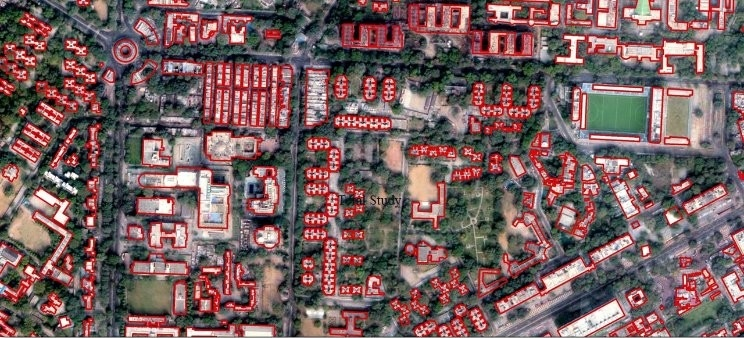
\includegraphics[width=\linewidth]{Figures/urban_planning_cropped.jpg} \\
        \small{Urban Planning}
      \end{center}
    \end{column}
  \end{columns}
\end{frame}



\begin{frame}[t]
  \frametitle{Introduction}
  In remote sensing images the objects are small fraction of the pixels of the image, qualifying this process as Small Object Detection. \\
  \vspace{0.5cm}
  Compared with large and medium objects, small objects are more difficult to detect accurately for the following reasons:
  \begin{itemize}
    \item Small objects have low resolution and insufficient features
    \item The span of object-scale is large and multiple scales coexist
    \item The examples of small objects are scarce
    \item Categories for small objects are imbalanced for the majority of datasets
  \end{itemize}
\end{frame}


\begin{frame}[t]
  \frametitle{Introduction}
  There are two ways to define small objects in the context of object detection.
  \begin{itemize}
    \item Relative size, where the bounding box of a small object should cover less than 1\% of the original image
    \item Absolute size, where a small object has size less than 32x32 pixels defined in MS-COCO dataset or 16x16 pixels defined in USC-GRAD-STDdb 
  \end{itemize} 

\end{frame}


\section{Data and Data Preprocessing}
\begin{frame}[t]
  \frametitle{Data and Data Preprocessing}
  The selected datasets cover a wide range of applications, from real-life scenarios to military and intelligence uses, ensuring a comprehensive evaluation 
  of the detection models.

  \begin{itemize}
    \item \href{https://cocodataset.org/}{Microsoft Common Object in COntext dataset}
    \item \href{https://github.com/VisDrone/VisDrone-Dataset}{Vis-Drone dataset}
    \item \href{https://www.kaggle.com/datasets/sovitrath/uav-small-object-detection-dataset}{Unmaned Arieal Vehicles - Small Object detection dataset}
  \end{itemize}
\end{frame}

% COCO
\begin{frame}[t]
  \frametitle{COCO2017 Dataset}
  The COCO2017 dataset includes complex everyday scenes with common objects in their natural context. It features:
  \begin{columns}
    \begin{column}{0.5\textwidth}
      \begin{itemize}
        \item 80 object categories
        \item 118.000 training images
        \item 5.000 validation images
        \item 41.000 test images 
        \item 1.5 million object instances
        \item Bounding boxes format: $[x_{center}, y_{center}, height, width]$
        \item Masks for objects provided
        \item Annotation format: Text format
      \end{itemize}
    \end{column}

    \begin{column}{0.5\textwidth}
      \centering
      \begin{figure}
        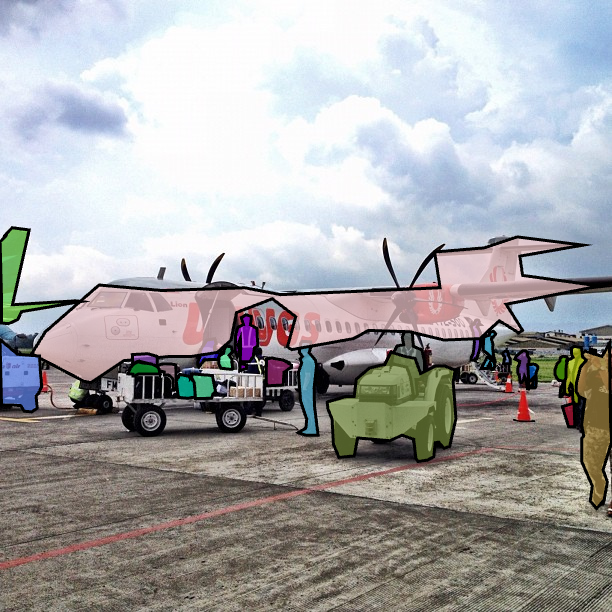
\includegraphics[scale=0.2]{Figures/coco-example.png}
        \caption{VisDrone sample}
        \label{fig:coco-ex}
      \end{figure}
    \end{column}
  \end{columns}

\end{frame}

\begin{frame}[t]
  \frametitle{COCO2017 Dataset}
  This dataset is used for object detection, segmentation, and captioning tasks. The class distribution of the dataset can be seen below:
  \begin{figure}[h!]
    \centering
    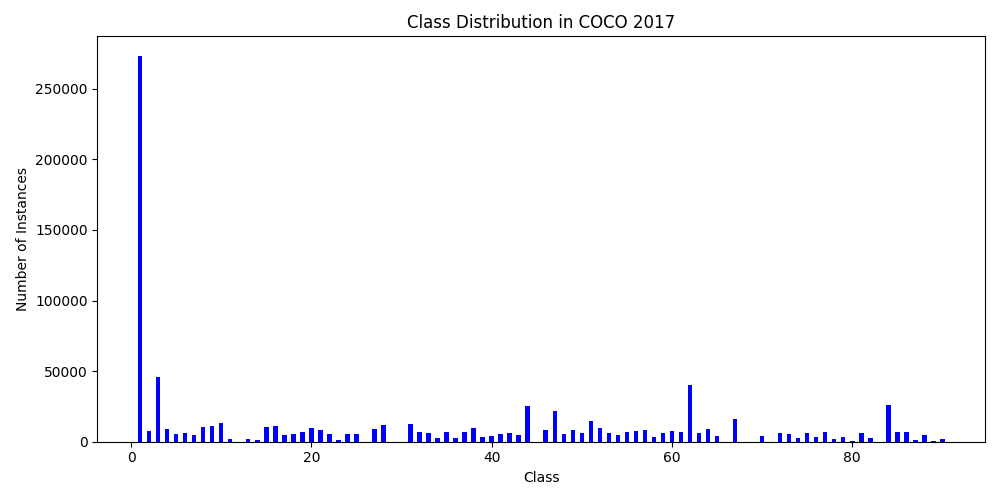
\includegraphics[scale=0.45]{Figures/coco2017_class_distribution.png}
    \caption{Class Distribution in COCO 2017}
    \label{fig:coco-class}
  \end{figure}
\end{frame}


% Vis
\begin{frame}[t]
  \frametitle{Vis-Drone Dataset}
  Vis-Drone is designed for drone-based image analysis and includes:

  \begin{columns}
    \begin{column}{0.5\textwidth}
      \begin{itemize}
        \item 10 object categories
        \item 6.471 training images, 
        \item 1.610 validation images
        \item 2.6 million object instances
        \item Bounding boxes format: $[x_{center}, y_{center}, height, width]$
        \item Masks for objects not provided
        \item Annotation format: Text format
      \end{itemize}
    \end{column}

    \begin{column}{0.5\textwidth}
      \centering
      \begin{figure}
        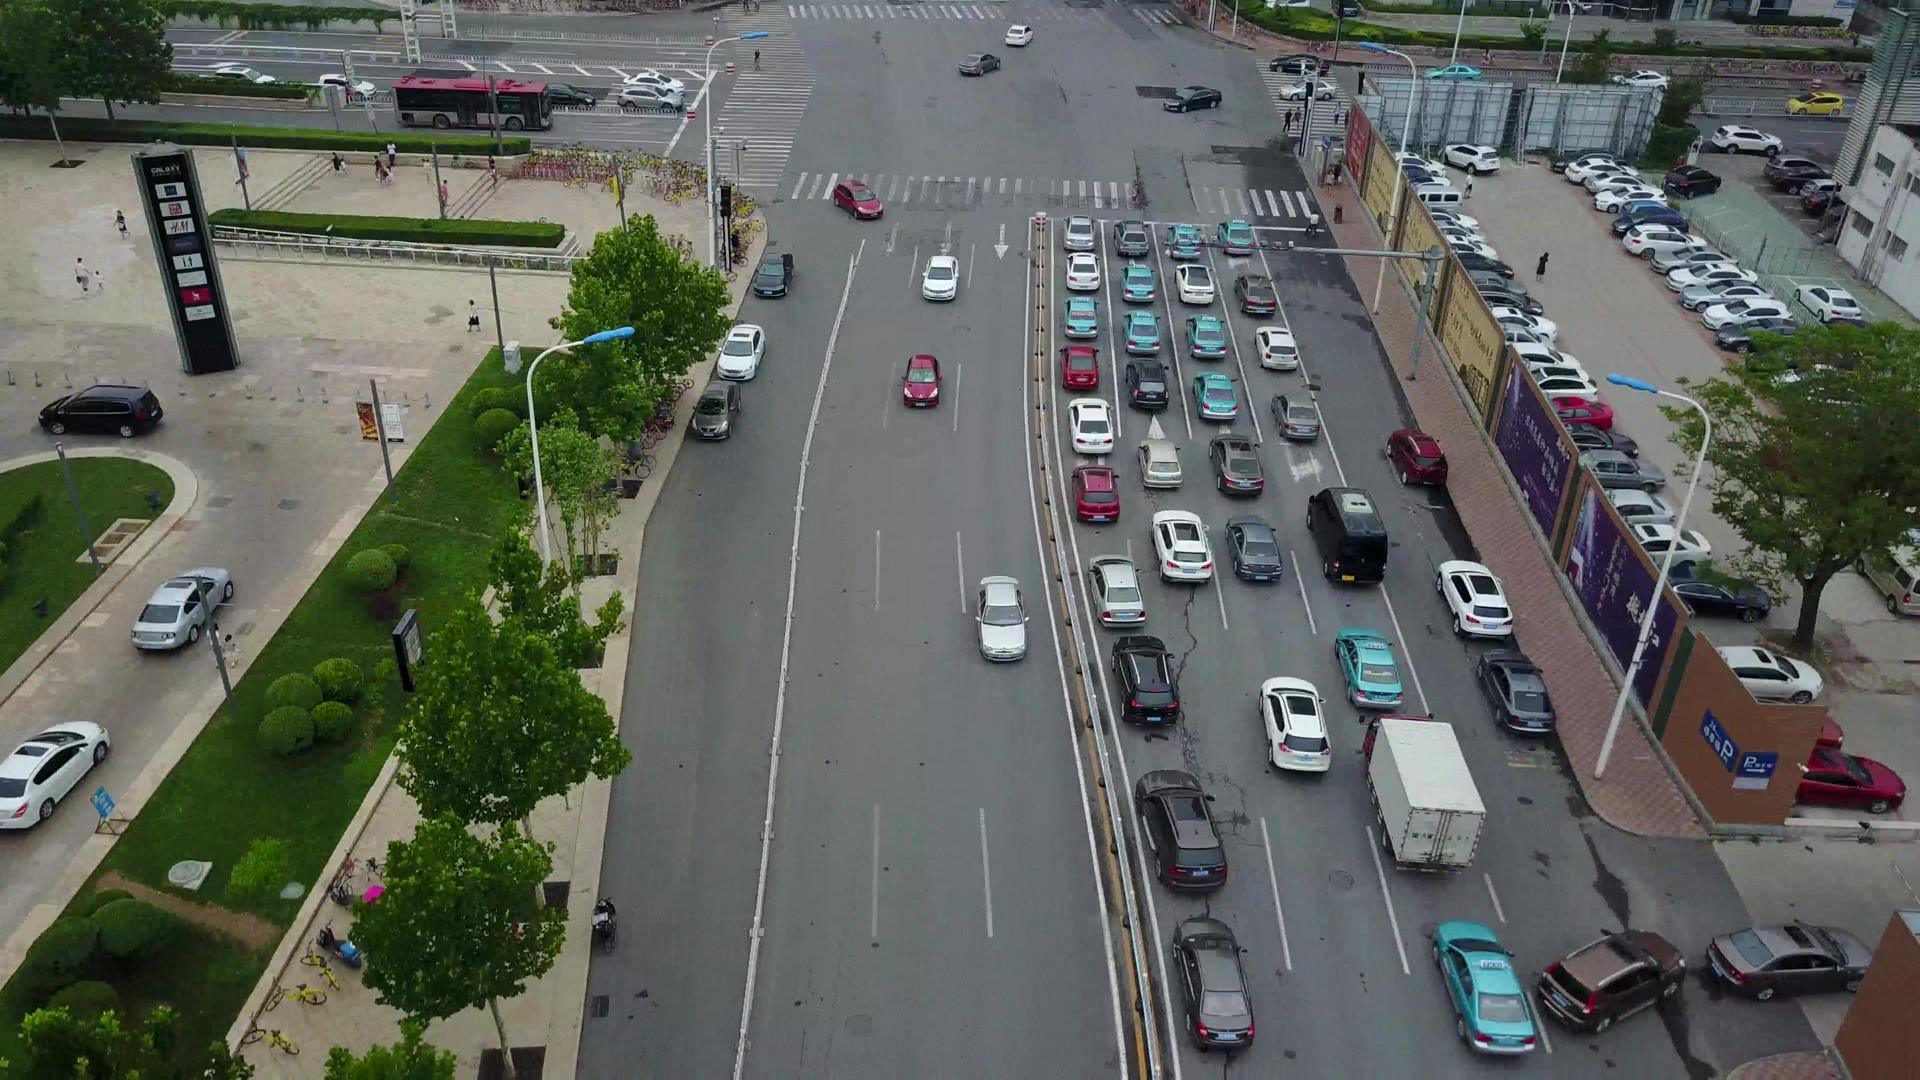
\includegraphics[scale=0.085]{Figures/vis_example.jpg}
        \caption{VisDrone sample}
        \label{fig:vis-ex}
      \end{figure}
    \end{column}
  \end{columns}
\end{frame}


\begin{frame}[t]
  \frametitle{Vis-Drone Dataset}
  This dataset is used mainly for small object detection and segmentation tasks. The class distribution of the dataset can be seen below:
  \begin{figure}[h!]
    \centering
    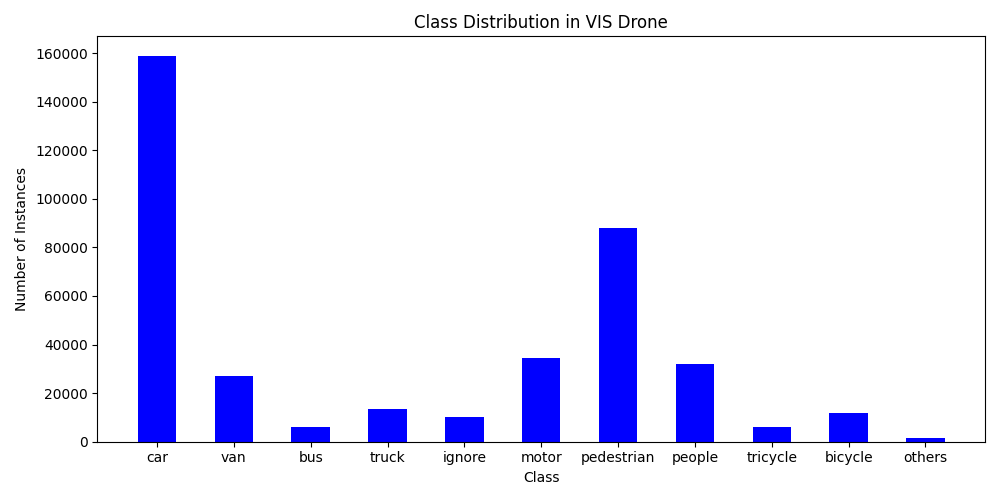
\includegraphics[scale=0.45]{Figures/vis_drone_data_class_distribution.png}
    \caption{Class Distribution in Vis-Drone}
    \label{fig:vis-class}
  \end{figure}
\end{frame}


% UAV
\begin{frame}[t]
  \frametitle{UAV-SOD Dataset}
  The UAV-SOD dataset is targeted at small object detection from aerial perspectives, featuring:
  \begin{columns}

    \begin{column}{0.5\textwidth}
      \begin{itemize}
        \item 10 object categories
        \item 717 training images 
        \item 84 validation images
        \item 43 test images 
        \item 18.234 object instances
        \item Bounding boxes format: $[x_{min}, y_{min}, x_{max}, y_{max}]$
        \item Masks for objects not provided
        \item Annotation format: XML format
      \end{itemize}
    \end{column}

    \begin{column}{0.5\textwidth}
      \centering
      \begin{figure}
        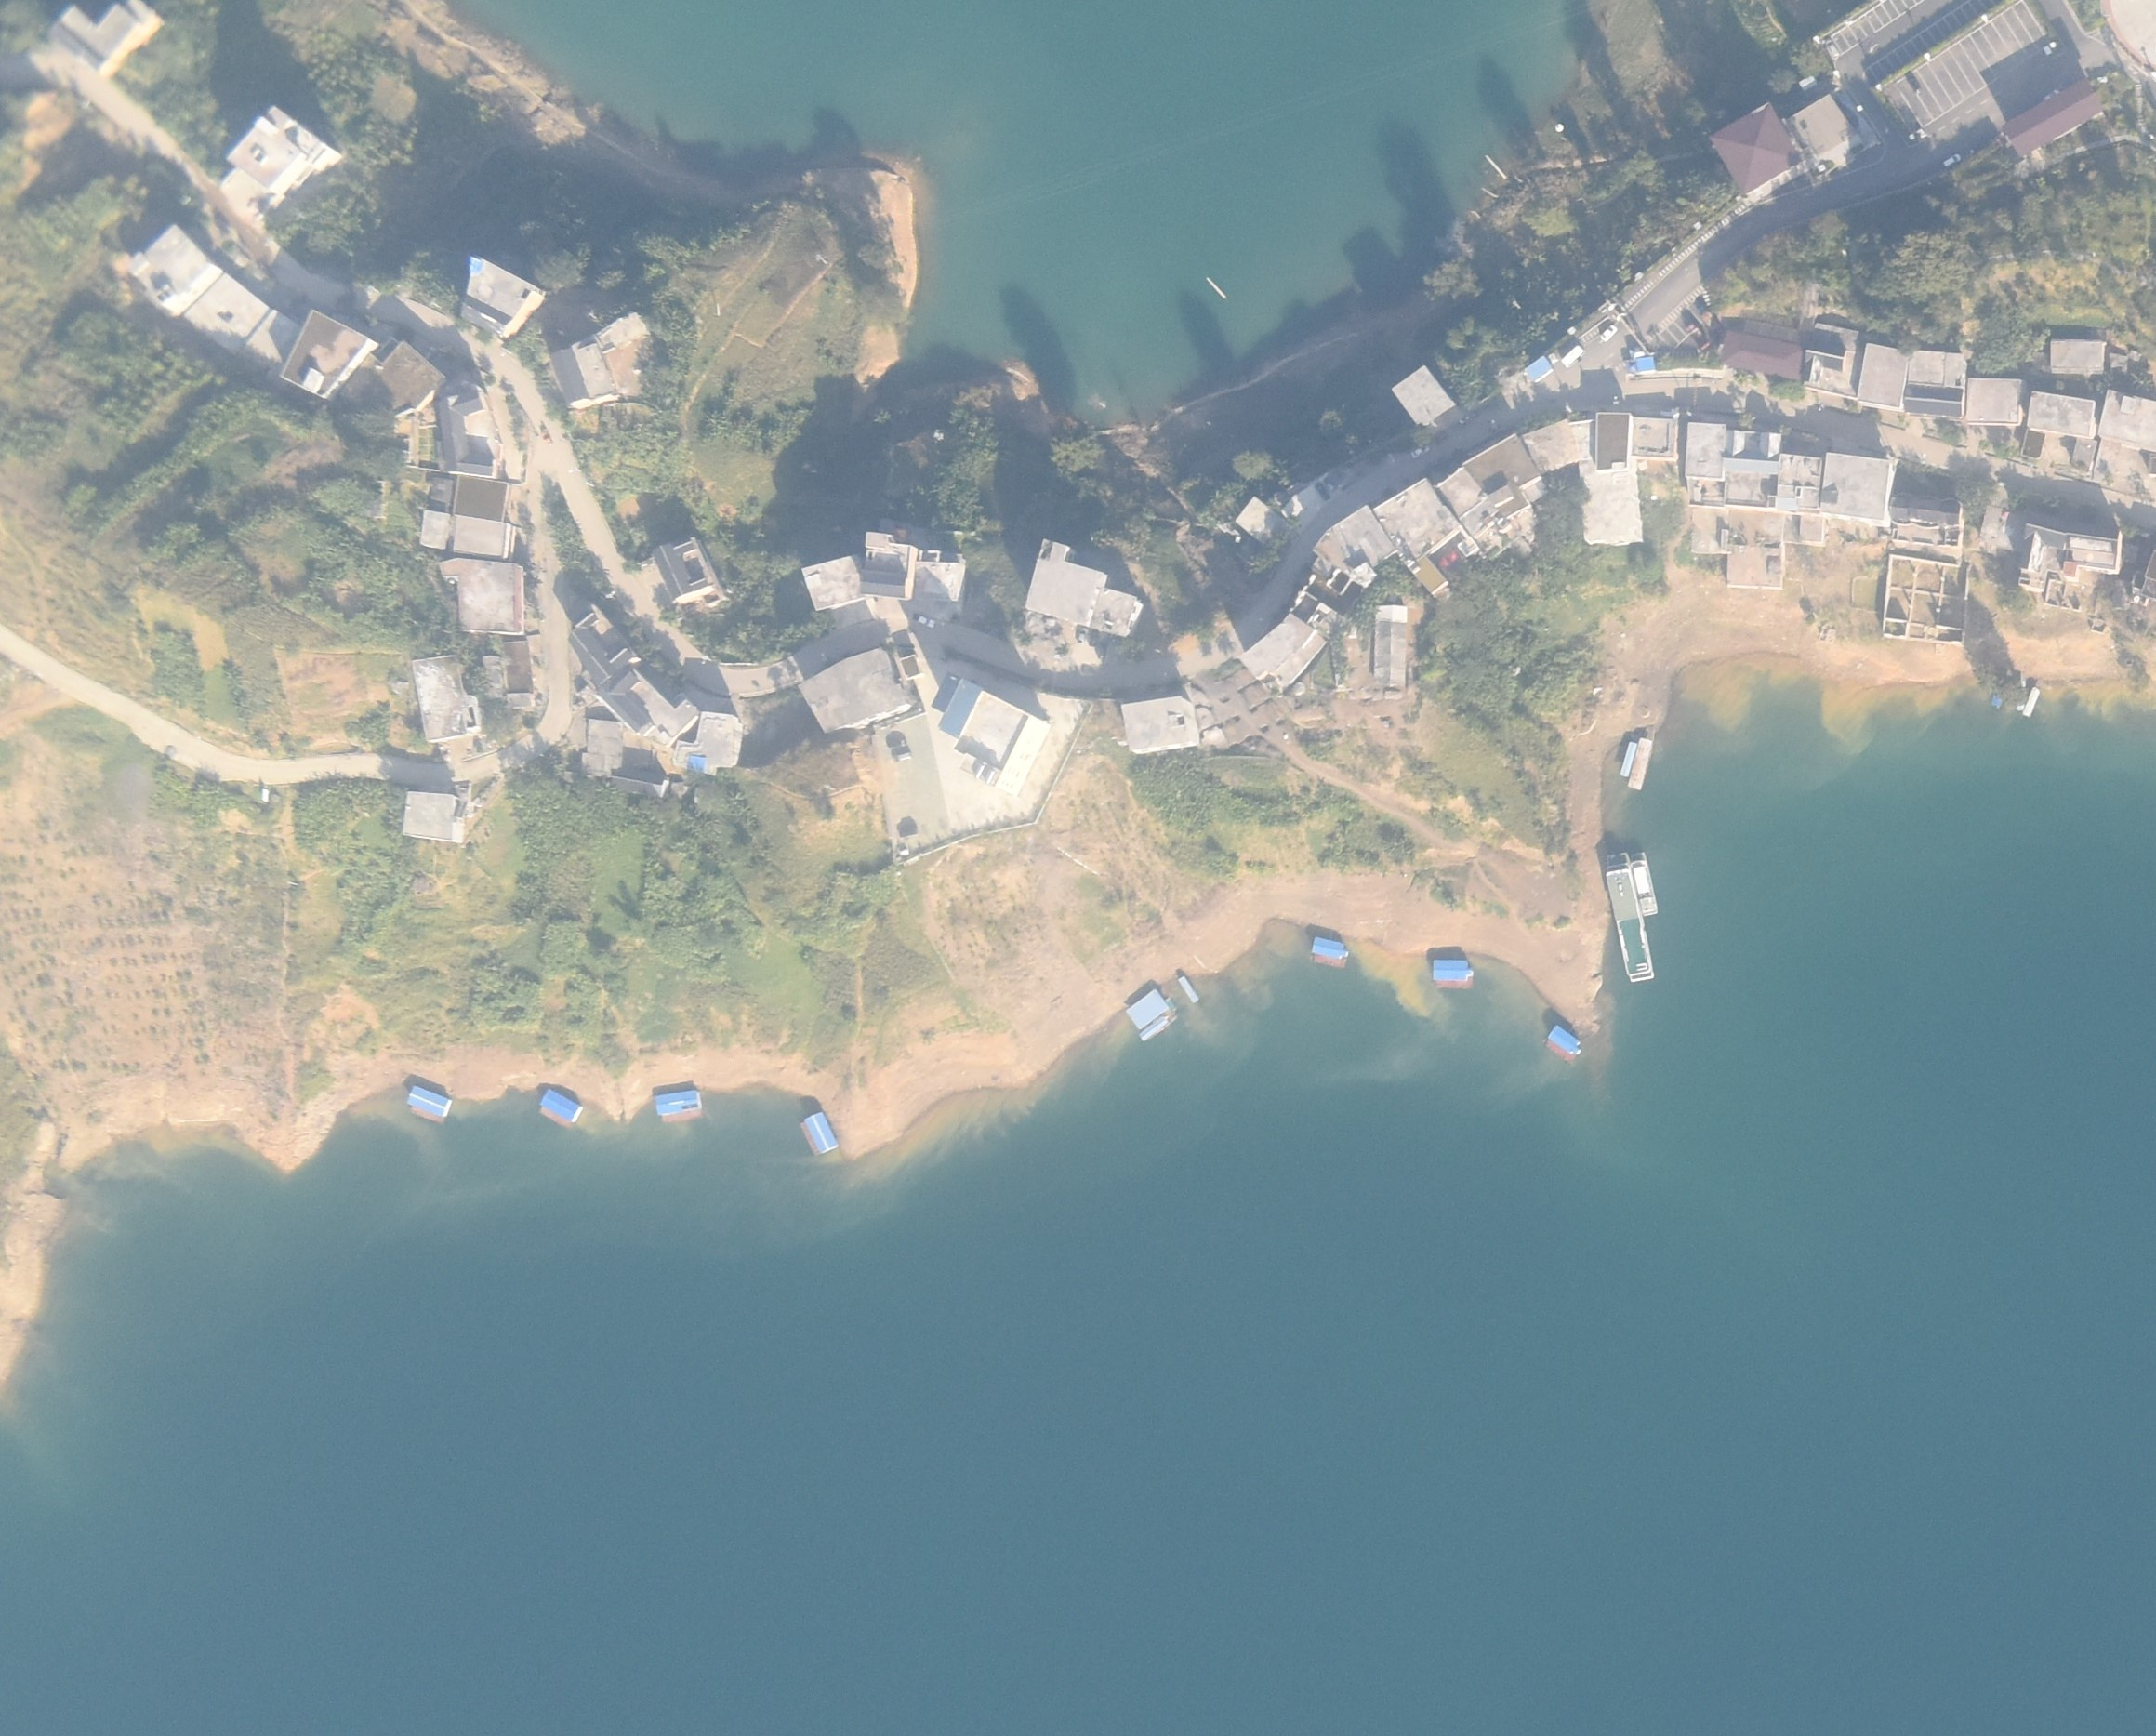
\includegraphics[scale=0.065]{Figures/uav_example2.jpg}
        \caption{UAV-SOD sample}
        \label{fig:uav-ex}
      \end{figure}
    \end{column}
  \end{columns}
\end{frame}




\begin{frame}[t]
  \frametitle{UAV-SOD Dataset}
  This dataset is used mainly for small object detection. The class distribution of the dataset can be seen below:
  \begin{figure}[h!]
    \centering
    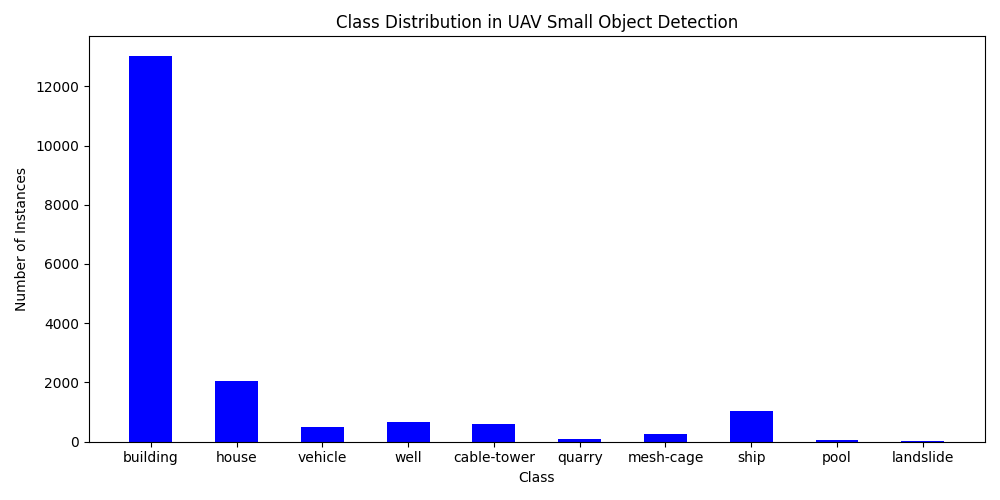
\includegraphics[scale=0.45]{Figures/uav_sod_data_class_distribution.png}
    \caption{Class Distribution in UAV-SOD}
    \label{fig:uav-class}
  \end{figure}
\end{frame}



\begin{frame}[t]
  \frametitle{Data Preprocessing Steps}
  Preprocessing is crucial for normalizing data and improving model training efficiency. Steps include:
  \begin{itemize}
    \item Resizing images and annotations to a uniform size of \(600 \times 600\) pixels.
    \item Image padding to maintain aspect ratio without distortion.
  \end{itemize}

  \begin{columns}
    \begin{column}{0.5\textwidth}
    \centering
    \begin{figure}
      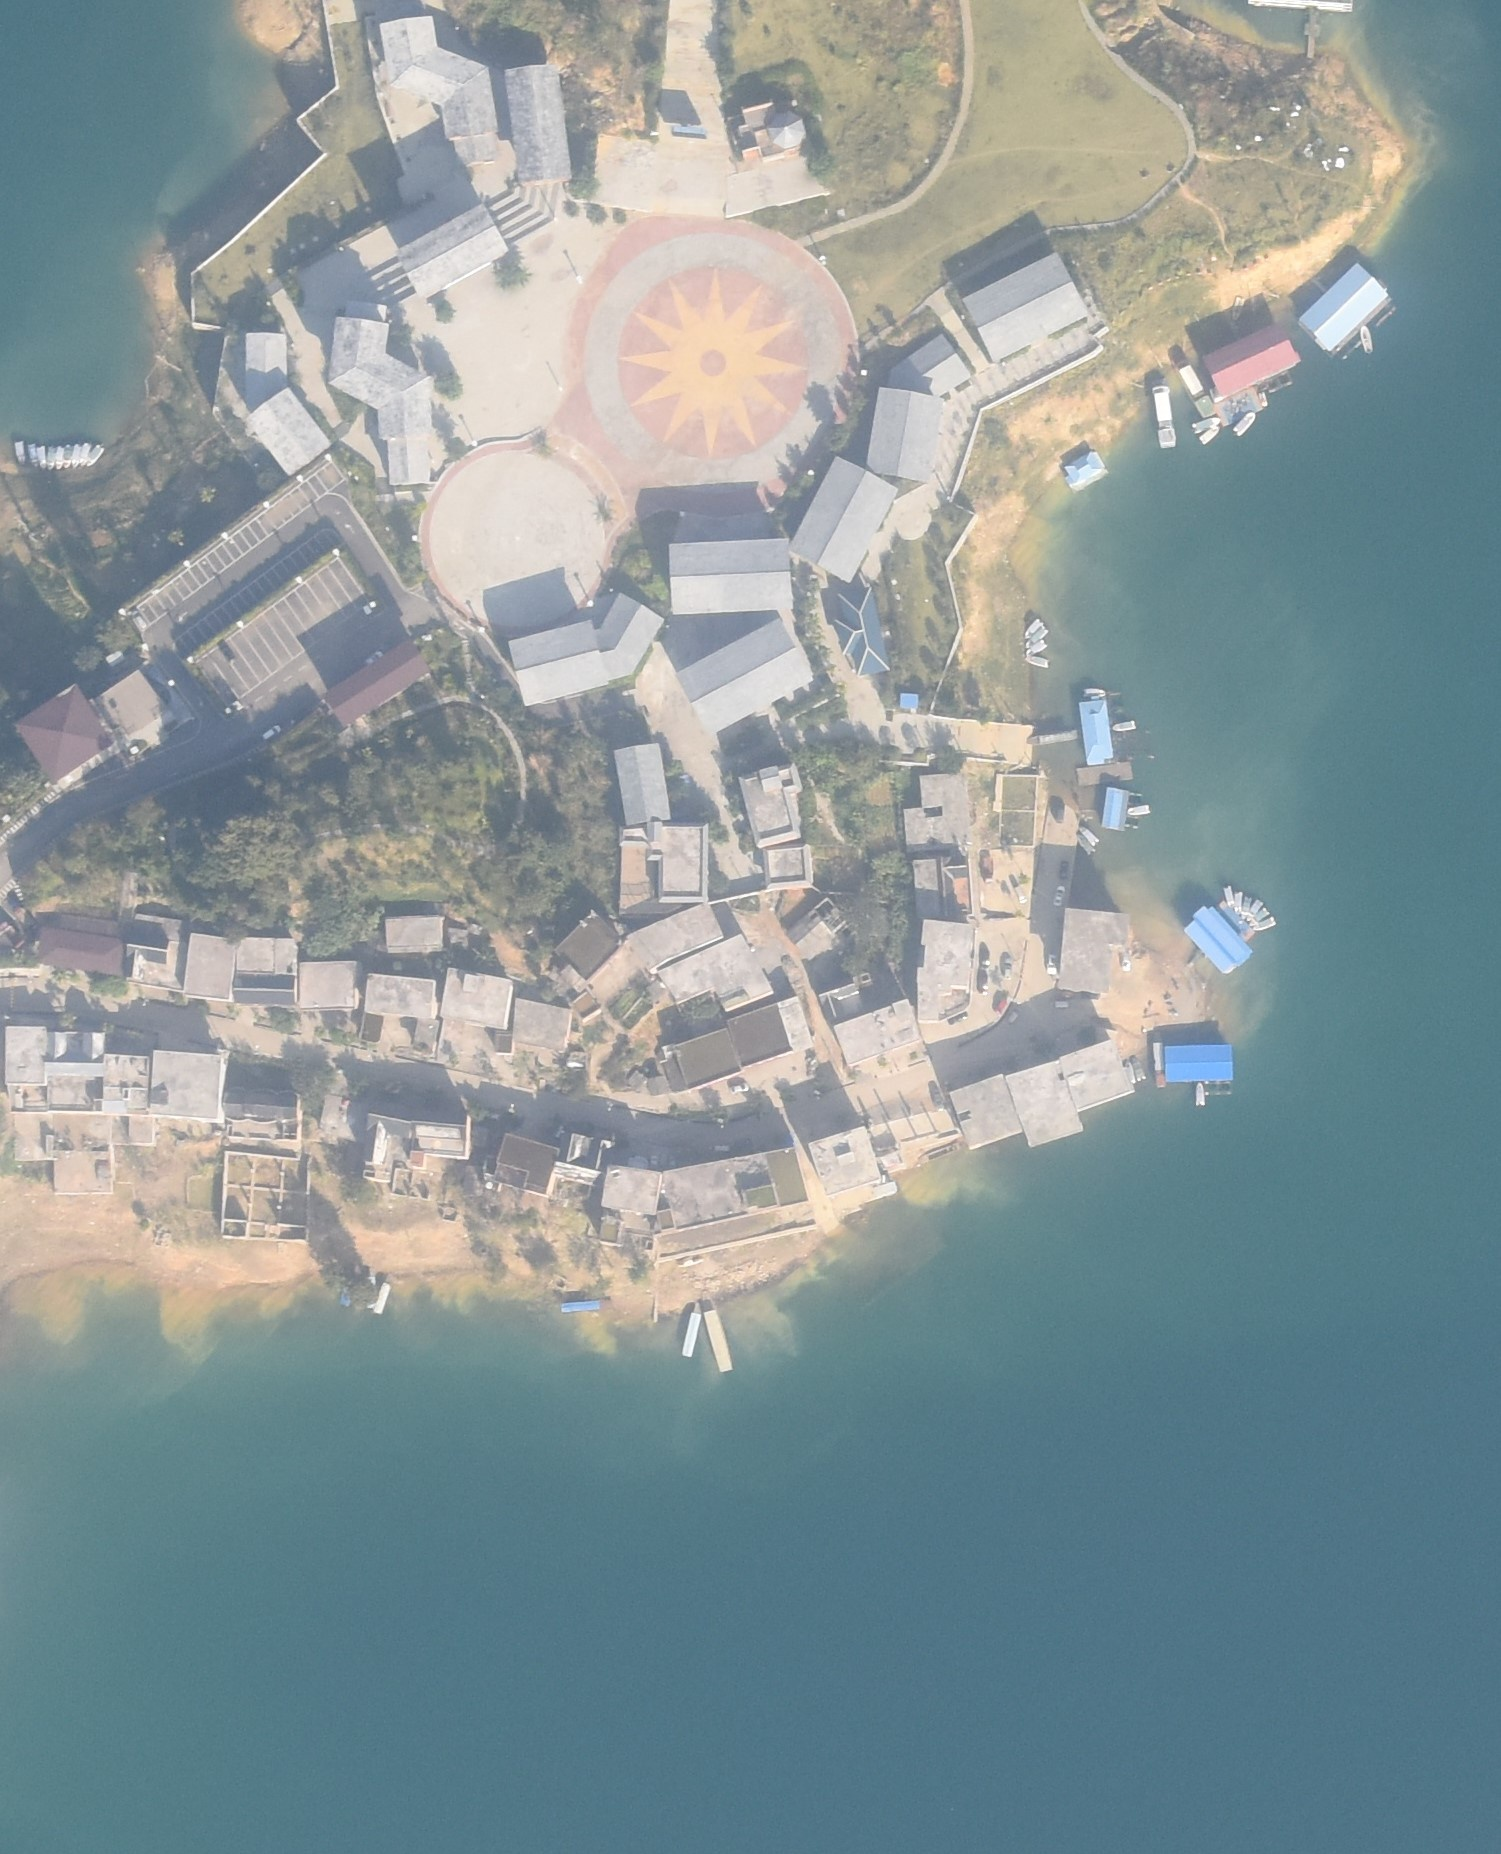
\includegraphics[scale=0.07]{Figures/uav_example.jpg}
      \caption{Image before Preprocessing}
      \label{fig:pre-process}
    \end{figure}
  \end{column}
  \begin{column}{0.5\textwidth}
    \centering
    \begin{figure}
      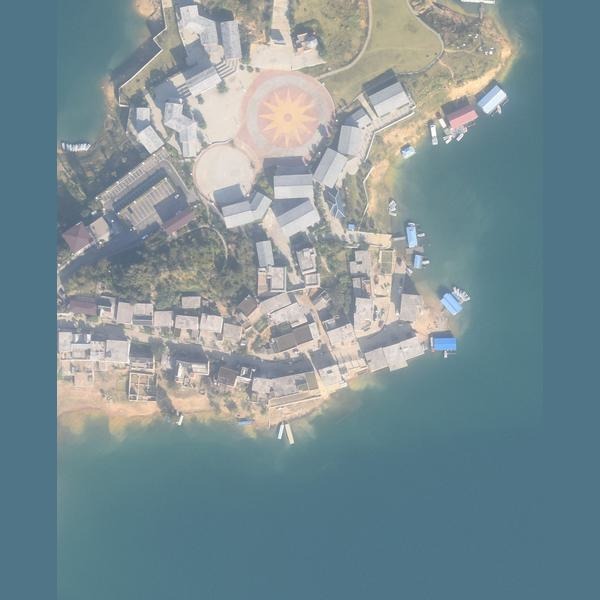
\includegraphics[scale=0.15]{Figures/uav_example_cropped.jpg}
      \caption{Image after Preprocessing}
      \label{fig:post-pre-process}
    \end{figure}
  \end{column}
\end{columns}

\end{frame}


\begin{frame}[t]
  \frametitle{Data Preprocessing Steps}
  \begin{itemize}
    \item Annotation format standardization for consistency across datasets.
    \item Normalization of image pixel values using dataset-specific mean and standard deviation.
    \item Create masks from bounding box coordinates.
  \end{itemize}
  \vspace{1cm}
  \textbf{Annotation Format Example:}
  \[x_{min}, y_{min}, x_{max}, y_{max}, class_{id}, [(x_1, y_1), (x_2, y_2), ..., (x_n, y_n)]\]

\end{frame}


\section{Object Detection Metrics}
\begin{frame}
  \frametitle{Object Detection Metrics: Precision and Recall}
  \textbf{Precision} - The proportion of true positive identifications made by the model out of all positive identifications it made.
  \[
  Precision = \frac{TP}{TP + FP}
  \]
  
  \textbf{Recall} - The proportion of true positive identifications made by the model out of all actual positives available during the test.
  \[
  Recall = \frac{TP}{TP + FN}
  \]
\end{frame}


\begin{frame}
  \frametitle{Object Detection Metrics: AP and mAP}
  \textbf{Average Precision (AP)} - A measure of precision across varying thresholds, reflecting the area under the precision-recall curve.
  \[
  AP = \sum_{n} (R_n - R_{n-1}) P_n
  \]
  
  \textbf{Mean Average Precision (mAP)} - The average of AP scores across all classes or varying IoU thresholds, providing a single overall effectiveness score for the detection system.
  \[
  mAP = \frac{1}{N} \sum_{i=1}^{N} AP_i
  \]
\end{frame}



\section{Proposed Method}
\begin{frame}
  \frametitle{Proposed Method}
  \begin{figure}[h!]
    \centering
    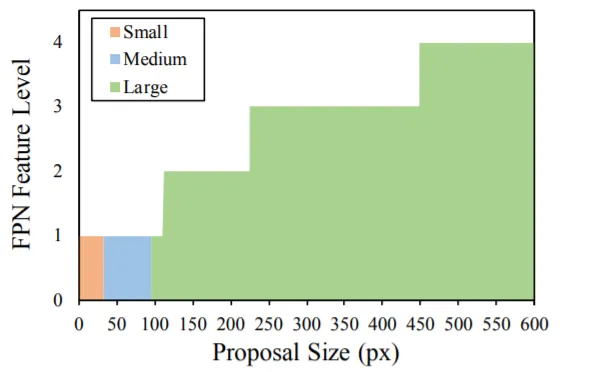
\includegraphics[scale=0.5]{Figures/efpn-sod-mapping.jpg}
    \caption{Object Detection Mapping}
    \label{fig:sod-problem}
  \end{figure}
\end{frame}

\begin{frame}
  \frametitle{Proposed Method}
  \begin{figure}[h!]
    \centering
    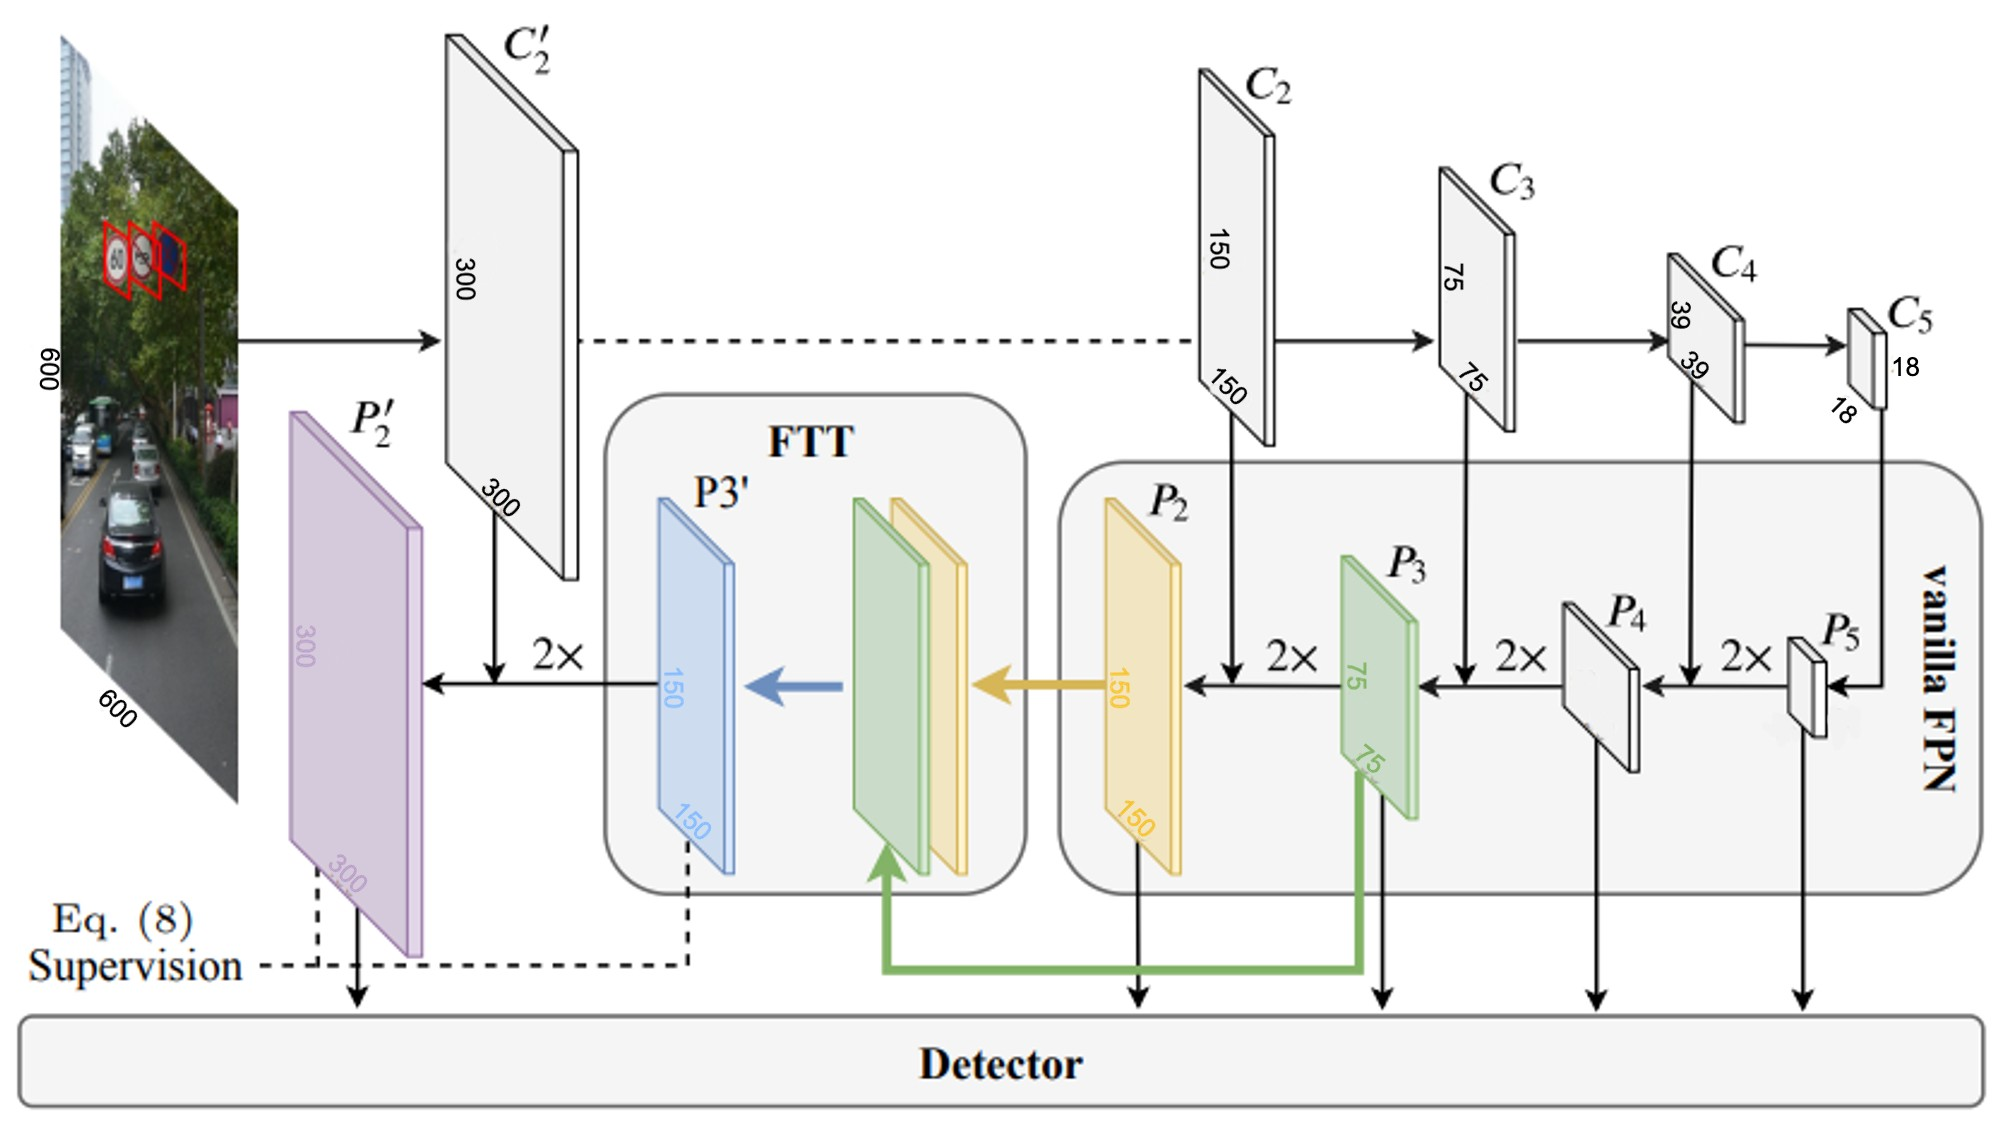
\includegraphics[scale=0.15]{Figures/efpn.jpg}
    \caption{Extended Feature Pyramid Network}
    \label{fig:efpn}
  \end{figure}
\end{frame}


\begin{frame}
  \frametitle{Proposed Method}
  \begin{figure}[h!]
    \centering
    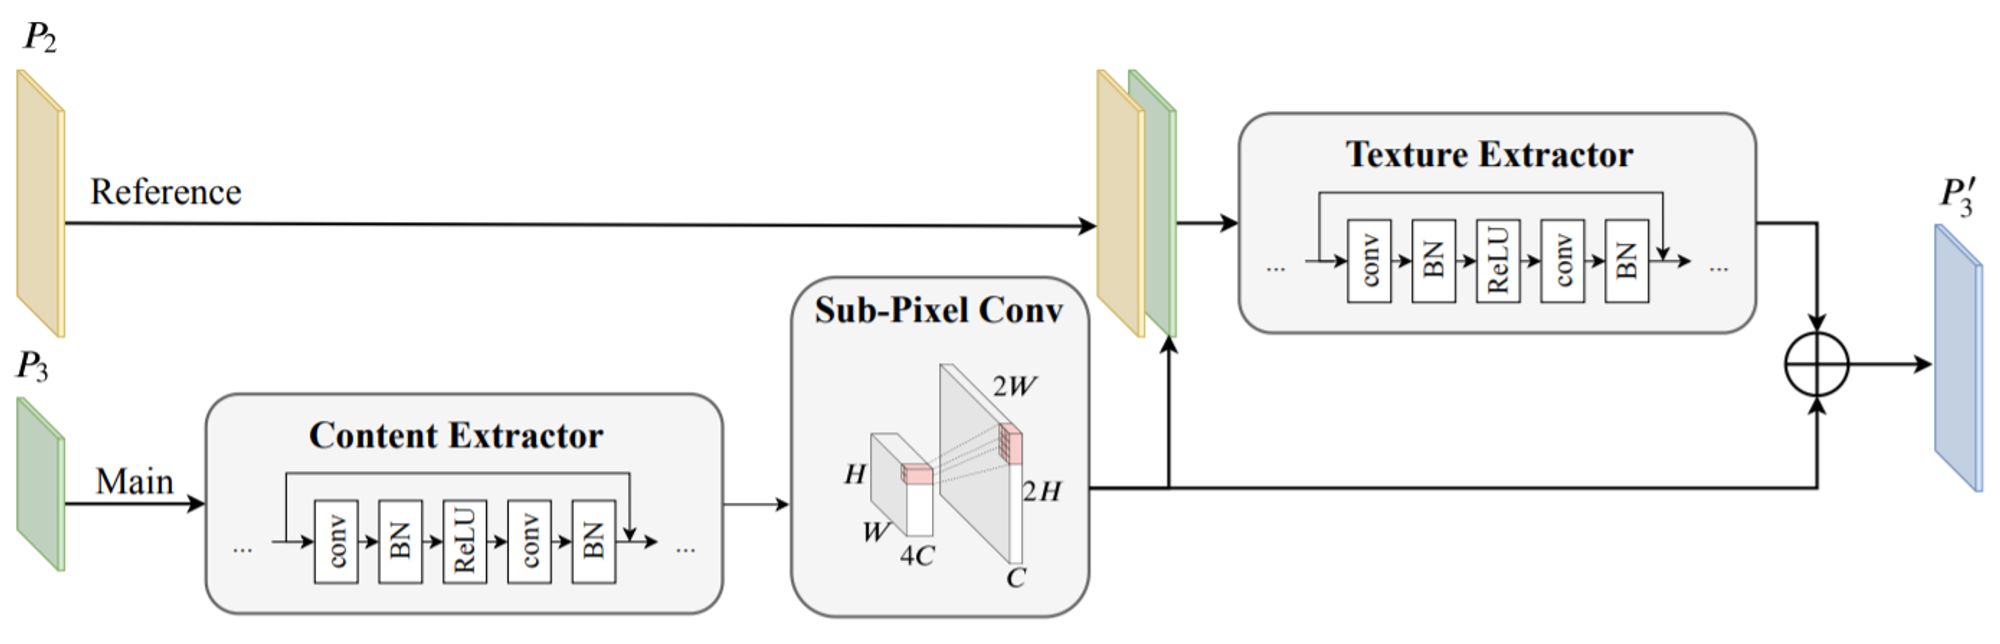
\includegraphics[scale=0.15]{Figures/ftt.png}
    \caption{Feature Texture Transfer}
    \label{fig:ftt}
  \end{figure}
\end{frame}

\begin{frame}
  \frametitle{Proposed Method}
  \begin{figure}[h!]
    \centering
    \includegraphics[scale=0.033]{Figures/EMAMT.png}
    \caption{Extended Masked-Attention Mask Transformer Architecture}
    \label{fig:proposed-model}
  \end{figure}
\end{frame}

\begin{frame}
  \frametitle{Proposed Method}
  \begin{figure}[h!]
    \centering
    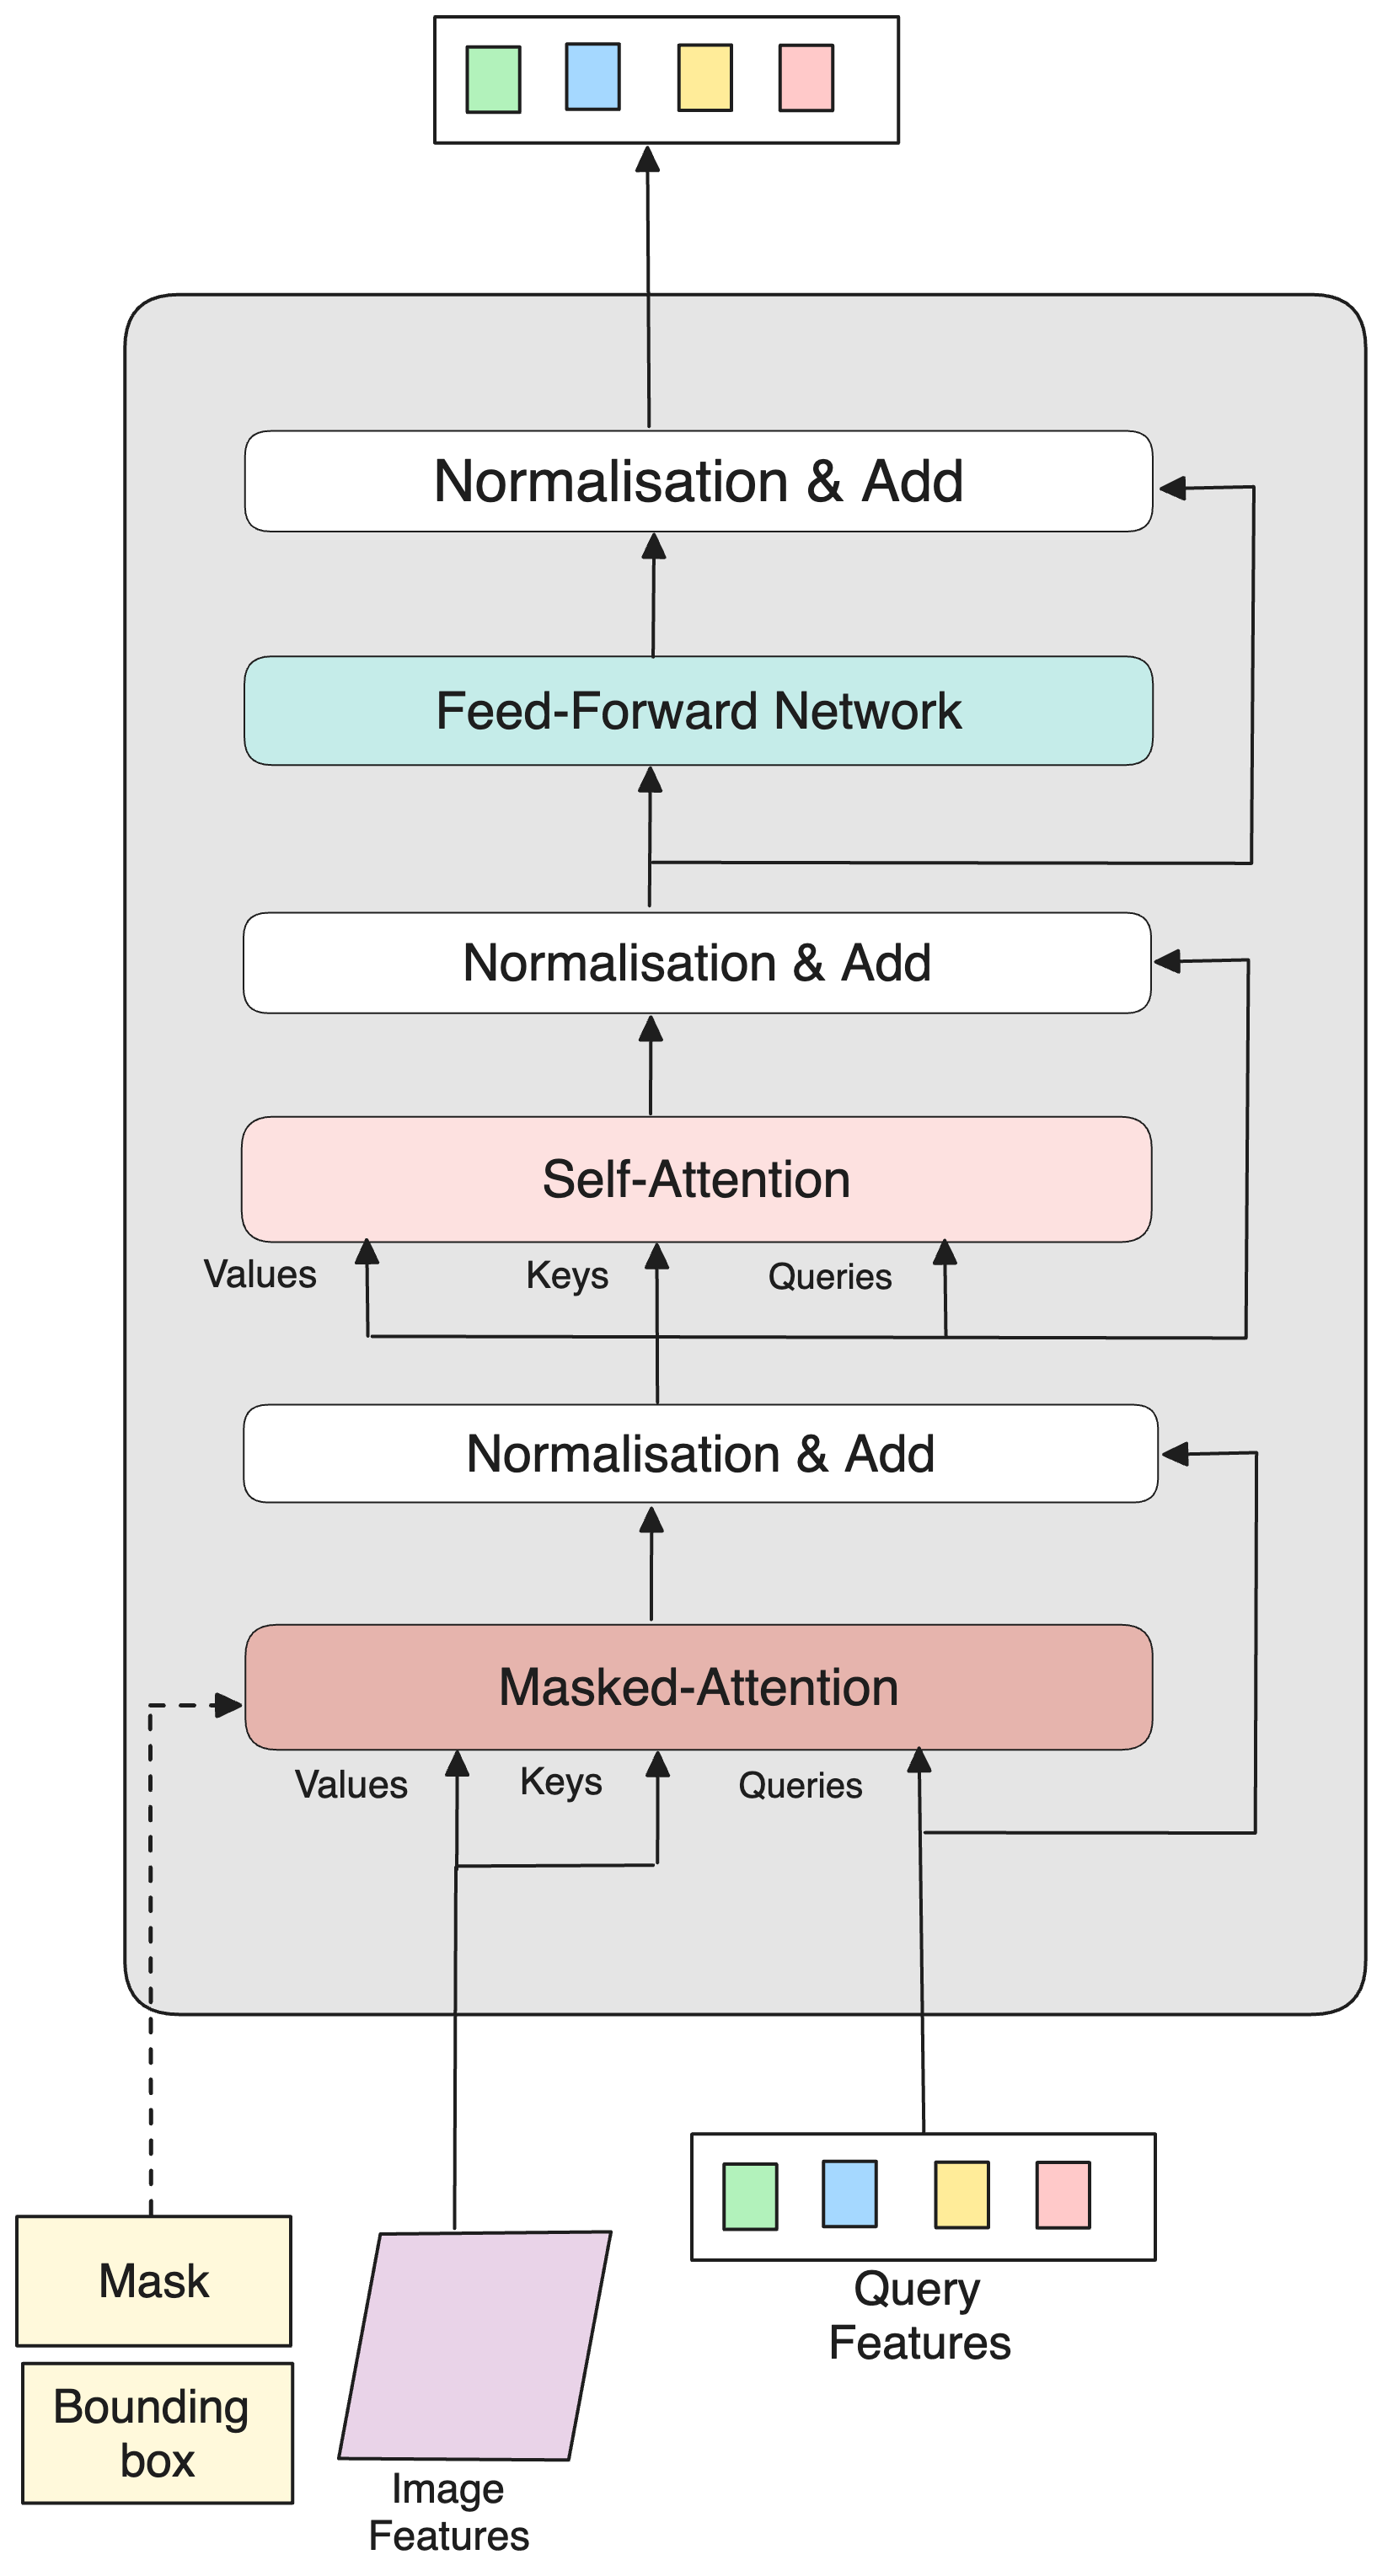
\includegraphics[scale=0.065]{Figures/emamt-decoder.png}
    \caption{Vision Transformer Architecture}
    \label{fig:proposed-model-Transformer}
  \end{figure}
\end{frame}

\begin{frame}[t]
  \frametitle{Proposed Method}
  To jointly optimize object detection and instance segmentation by incorporating multiple loss components, each addressing specific aspects of model 
  performance.

  \[L_{total} = \lambda_{mask} L_{mask} + \lambda_{bbox} L_{bbox} + \lambda_{class} L_{class}\]

  \begin{itemize}
    \item Mask Loss - \(\lambda_{mask} = 1\)
    \item Bounding Box Loss - \(\lambda_{bbox} = 1\)
    \item Class Loss - \(\lambda_{class} = 0.8\)
  \end{itemize}

\end{frame}

\section{Experiments}
\begin{frame}[t]
  \frametitle{Experiments}
  To effectively implement and evaluate the Extended Masked-Attention Mask Transformer, we utilized Amazon Web Services (AWS) SageMaker, 
  leveraging the powerful \textit{ml.p4d.24xlarge} instance with eight NVIDIA A100 GPUs.

  \vspace{1cm}
  
  The table below summarizes the tailored training parameters per dataset, optimized through extensive experimentation to maximize model performance.

  \begin{table}[h]
    \scriptsize
    \centering
    \begin{tabular}{|c|c|c|c|}
        \hline
        &                   \textbf{MS COCO}      & \textbf{UAV-SOD}     & \textbf{VisDrone}            \\ \hline
        Number of Epochs   & 125                  & 75                   & 75                           \\ \hline
        Optimizer          & AdamW                & AdamW                & AdamW                        \\ \hline
        Learning Rate      & $1 \times 10^{-4}$   & $1 \times 10^{-3}$   & $1 \times 10^{-3}$           \\ \hline
        Batch size         & 4                    &  4                   & 4                            \\ \hline
        Image size         & $600\times600$       &  $600\times600$      & $600\times600$               \\ \hline
        Number of Anchors  & $30000$              &  $722$               & $722$                        \\ \hline
    \end{tabular}
    \caption{Details of training parameters per dataset}
    \label{tab:training_parameters}
  \end{table}
\end{frame}



\begin{frame}[t]
  \scriptsize
  \frametitle{Experiments - COCO2017}
  \begin{figure}[h!]
    \centering
    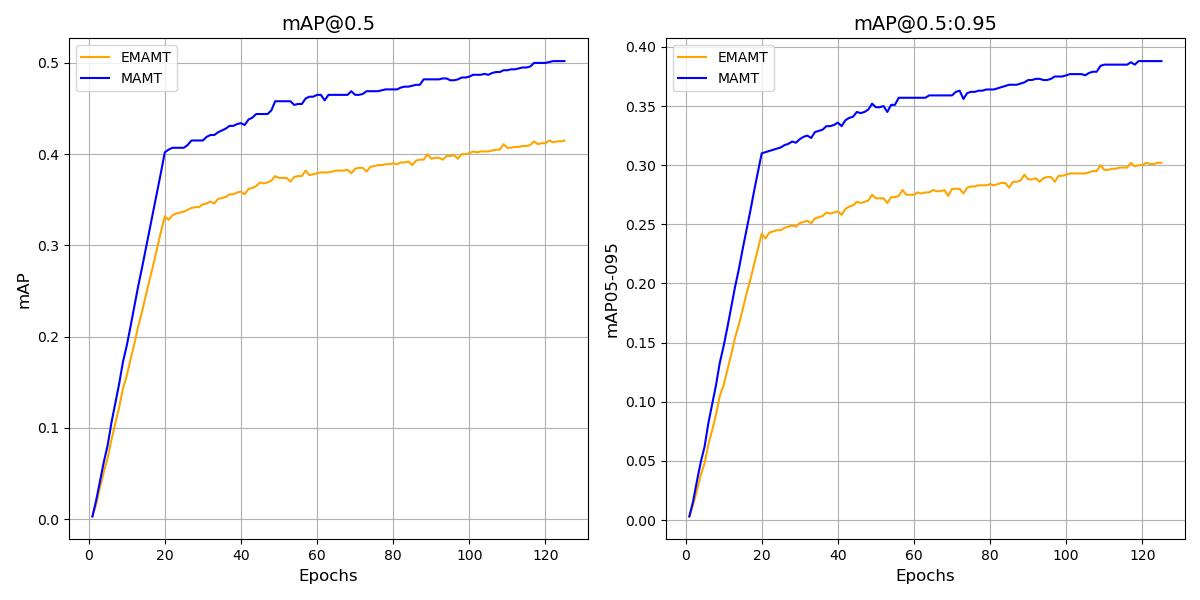
\includegraphics[scale=0.25]{Figures/coco_train.jpg}
    \caption{Performance comparison of MAMT and EMAMT on mAP at 50\% IoU threshold (left) and the average mAP across IoU thresholds from 50\% to 95\% (right) 
    for the COCO2017 dataset}
    \label{fig:coco-train}
  \end{figure}


  \begin{table}[h]
    \centering
    \begin{tabular}{|c|c|c|c|c|c|}
        \hline
        \textbf{Model}     & \textbf{mAP(@0.5)}     & \textbf{mAP(@0.5:0.95)}    & \textbf{Queries}   & \textbf{Parameters} & \textbf{GFLOPs}  \\ \hline
        EMAMT              & 44.5                   & 30.2                       & \textbf{100}       & \textbf{95M}        &  \textbf{492}     \\ \hline
        MAMT               & \textbf{50.2}          & \textbf{38.8}              & 200                & 216M                &  868              \\ \hline
    \end{tabular}
    \caption{Results for COCO dataset}
    \label{tab:coco_results}
  \end{table}
\end{frame}



\begin{frame}[t]
  \scriptsize
  \frametitle{Experiments - COCO2017}
  \begin{columns}
      \begin{column}{0.5\textwidth}
      \centering
      \begin{figure}
        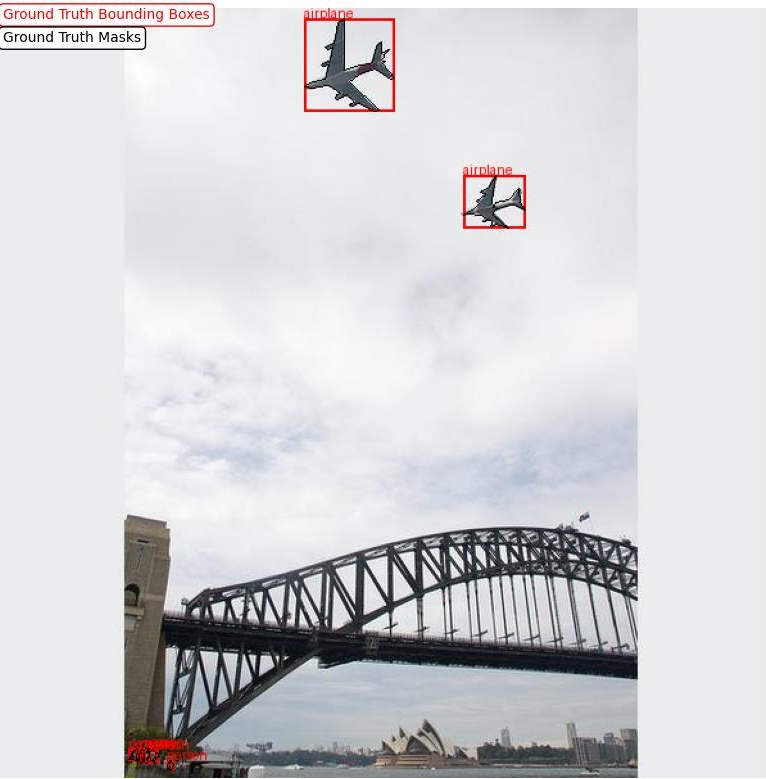
\includegraphics[scale=0.22]{Figures/coco_ground_truth.jpg}
        \caption{Image with Ground Truth Bounding Boxes and Masks}
        \label{fig:pre-process}
      \end{figure}
    \end{column}
    \begin{column}{0.5\textwidth}
      \centering
      \begin{figure}
        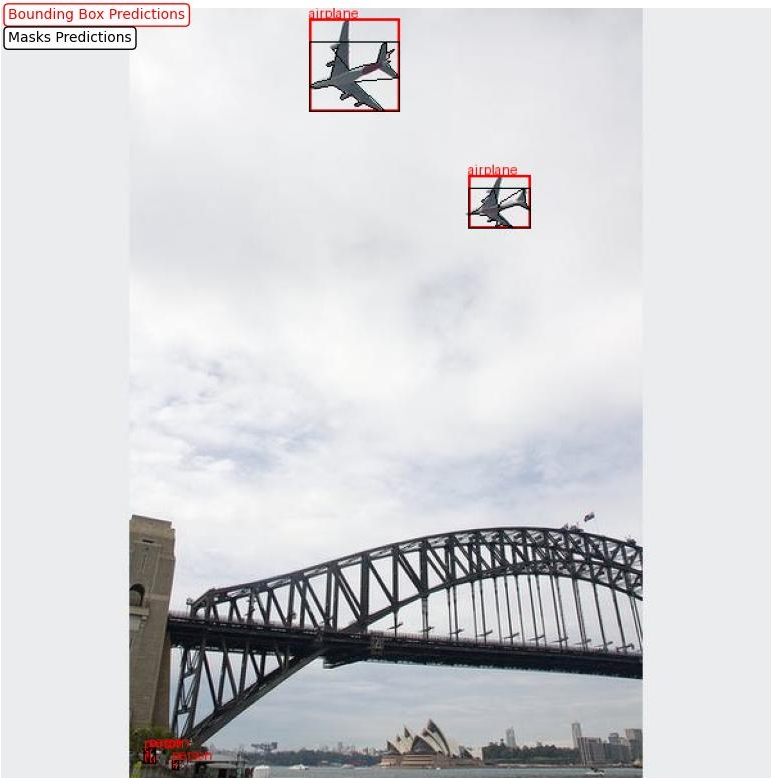
\includegraphics[scale=0.22]{Figures/coco_predictions.jpg}
        \caption{Image with Predicted Bounding Boxes and Masks}
        \label{fig:post-pre-process}
      \end{figure}
    \end{column}
  \end{columns}
\end{frame}


\begin{frame}[t]
  \scriptsize
  \frametitle{Experiments - VisDrone}

  \begin{figure}[h!]
    \centering
    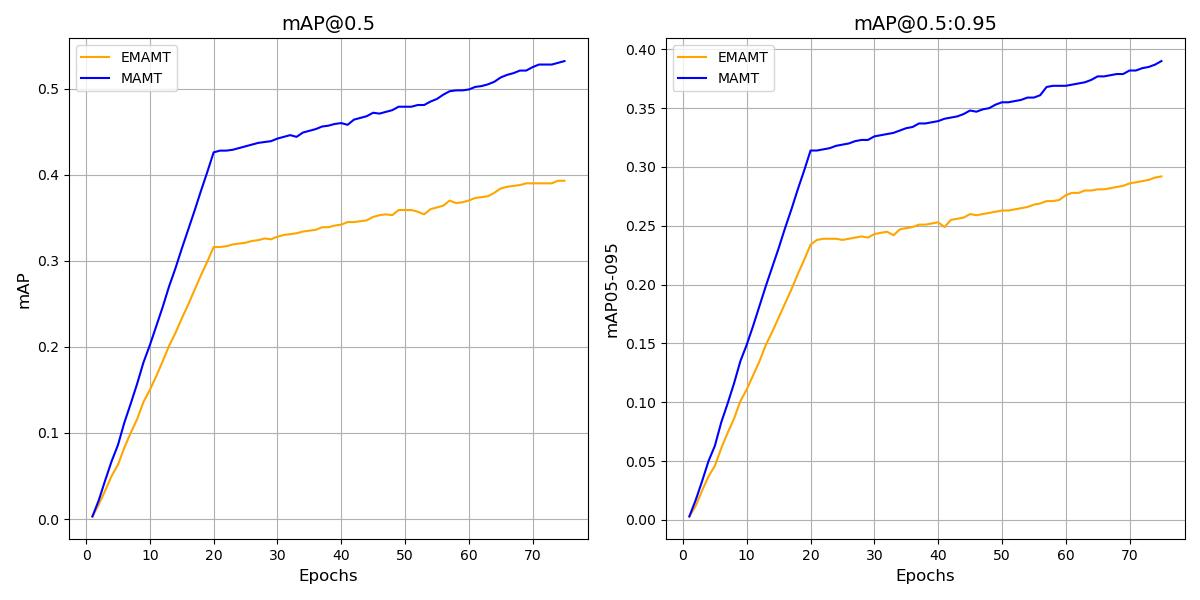
\includegraphics[scale=0.25]{Figures/vis_train.jpg}
    \caption{Performance comparison of MAMT and EMAMT on mAP at 50\% IoU threshold (left) and the average mAP across IoU thresholds from 50\% to 95\% (right) 
    for the VisDrone dataset}
    \label{fig:uav-train}
  \end{figure}

  \begin{table}[h]
    \centering
    \begin{tabular}{|c|c|c|c|c|c|}
        \hline
        \textbf{Model}     & \textbf{mAP(@0.5)}     & \textbf{mAP(@0.5:0.95)}    & \textbf{Queries}   & \textbf{Parameters} & \textbf{GFLOPs}  \\ \hline
        EMAMT              & 39.5                   & 29.2                       & \textbf{100}       & \textbf{95M}        &  \textbf{492}     \\ \hline
        MAMT               & \textbf{53.2}          & \textbf{39.2}              & 200                & 216M                &  868              \\ \hline
    \end{tabular}
    \caption{Results for VisDrone dataset}
    \label{tab:vis_results}
  \end{table}
\end{frame}


\begin{frame}[t]
  \scriptsize
  \frametitle{Experiments - VisDrone}
  \begin{columns}
      \begin{column}{0.5\textwidth}
      \centering
      \begin{figure}
        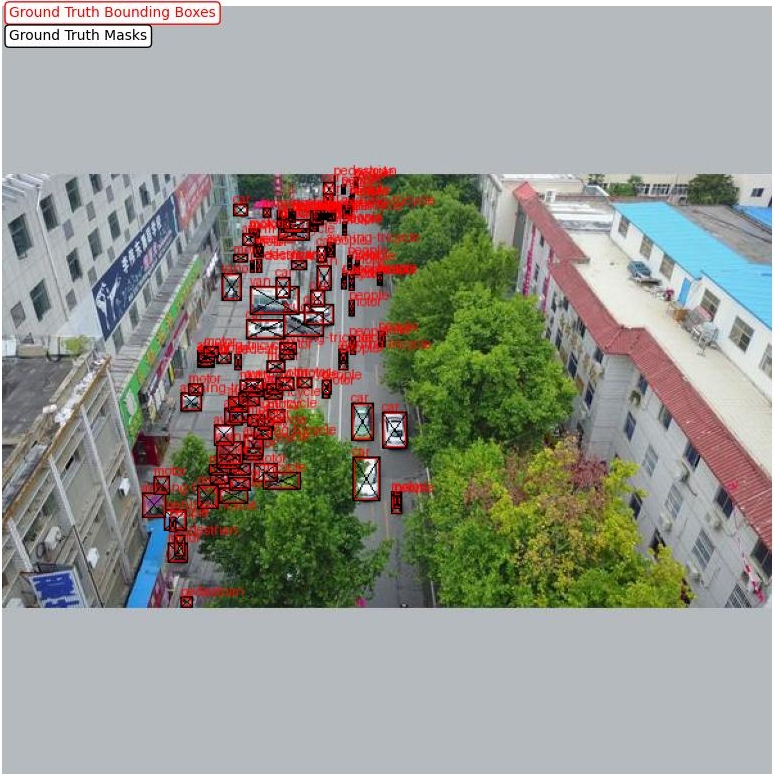
\includegraphics[scale=0.22]{Figures/vis_ground_truth.jpg}
        \caption{Image with Ground Truth Bounding Boxes and Masks}
        \label{fig:pre-process}
      \end{figure}
    \end{column}
    \begin{column}{0.5\textwidth}
      \centering
      \begin{figure}
        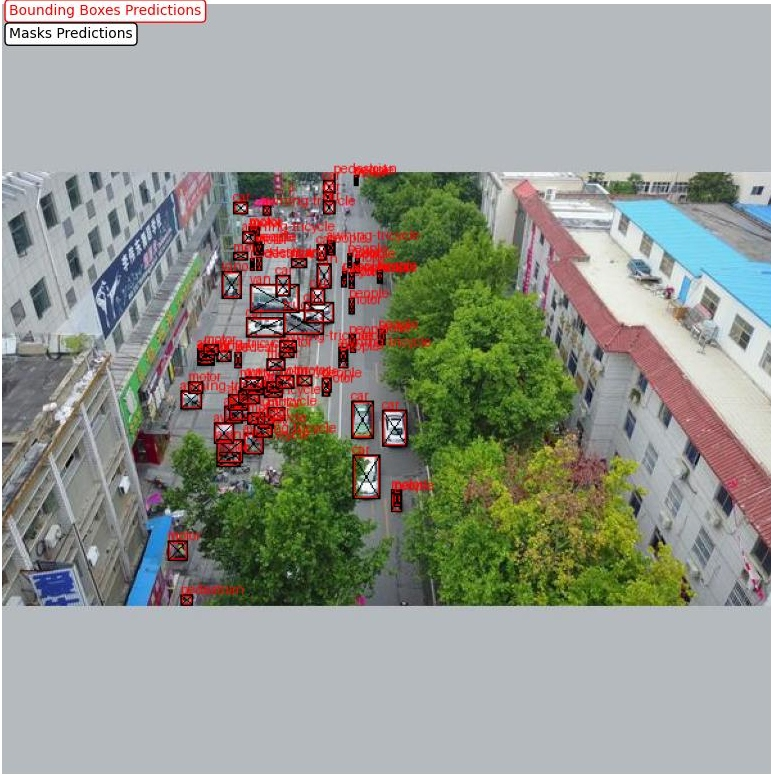
\includegraphics[scale=0.22]{Figures/vis_predictions.jpg}
        \caption{Image with Predicted Bounding Boxes and Masks}
        \label{fig:post-pre-process}
      \end{figure}
    \end{column}
  \end{columns}
\end{frame}


\begin{frame}[t]
  \scriptsize
  \frametitle{Experiments - UAV-SOD}

  \begin{figure}[h!]
    \centering
    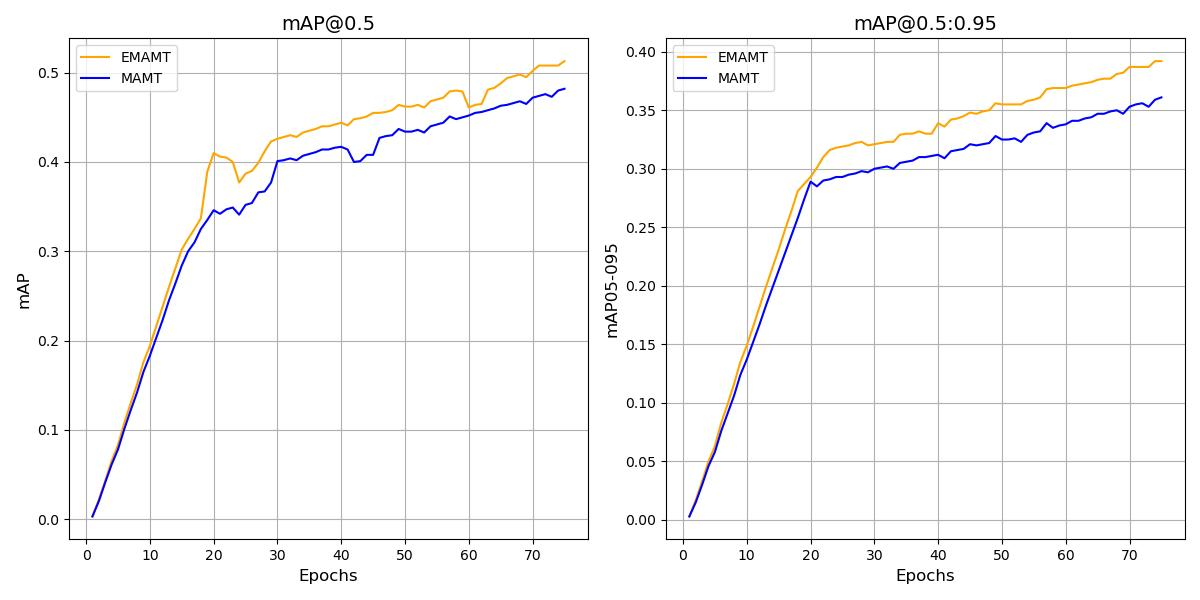
\includegraphics[scale=0.25]{Figures/uav_train.jpg}
    \caption{Performance comparison of MAMT and EMAMT on mAP at 50\% IoU threshold (left) and the average mAP across IoU thresholds from 50\% to 95\% (right) 
    for the UAV-SOD dataset}
    \label{fig:uav-train}
\end{figure}

  \begin{table}[h]
    \centering
    \begin{tabular}{|c|c|c|c|c|c|}
        \hline
        \textbf{Model}     & \textbf{mAP(@0.5)}    & \textbf{mAP(@0.5:0.95)}    & \textbf{Queries}   & \textbf{Parameters} & \textbf{GFLOPs}  \\ \hline
        EMAMT              & \textbf{51.3}         & \textbf{39.2}              & \textbf{100}       & \textbf{95M}        &  \textbf{492}     \\ \hline
        MAMT               & 48.2                  & 36.1                       & 200                & 216M                &  868              \\ \hline
    \end{tabular}
    \caption{Results for UAV-SOD dataset}
    \label{tab:uav_results}
  \end{table}
\end{frame}

\begin{frame}[t]
  \scriptsize
  \frametitle{Experiments UAV-SOD}
  \begin{columns}
      \begin{column}{0.5\textwidth}
      \centering
      \begin{figure}
        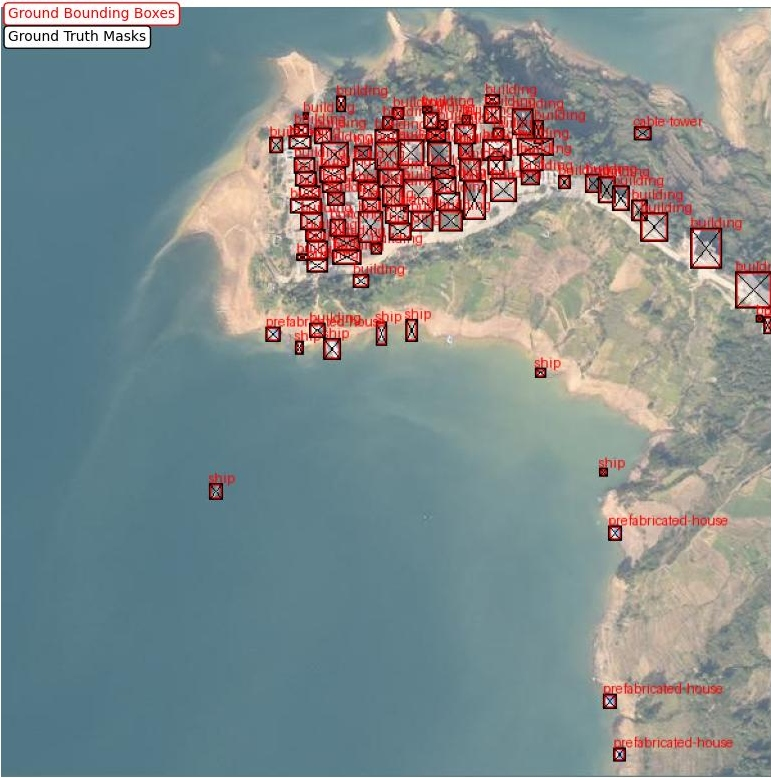
\includegraphics[scale=0.22]{Figures/uav_ground_truth.jpg}
        \caption{Image with Ground Truth Bounding Boxes and Masks}
        \label{fig:pre-process}
      \end{figure}
    \end{column}
    \begin{column}{0.5\textwidth}
      \centering
      \begin{figure}
        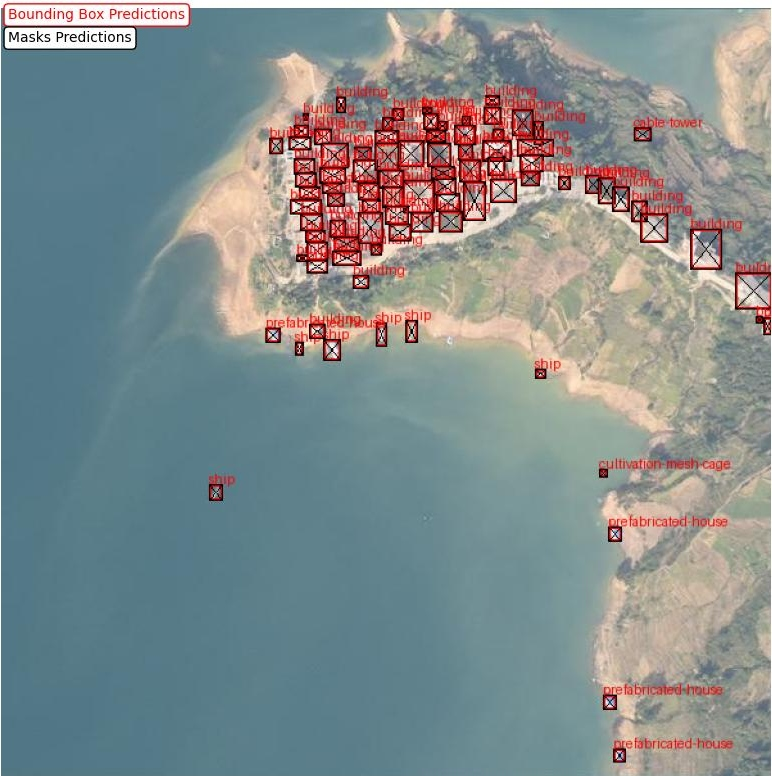
\includegraphics[scale=0.22]{Figures/uav_predictions.jpg}
        \caption{Image with Predicted Bounding Boxes and Masks}
        \label{fig:post-pre-process}
      \end{figure}
    \end{column}
  \end{columns}
\end{frame}


\section{Conclusion}
\begin{frame}[t]
  \frametitle{Conclusion: Overview and Achievements}
  We introduced the \textit{Extended Masked-Attention Mask Transformer (EMAMT)}, integrating the Enhanced Feature Pyramid Network (EFPN) with Mask2Former, aiming at enhanced efficiency and accuracy in object detection.

  \textbf{Key Findings:}
  \begin{itemize}
    \item EMAMT achieved up to 56\% reduction in model complexity compared to the traditional Masked-Attention Mask Transformer (MAMT).
    \item EMAMT surpassed MAMT in performance on the UAV-SOD dataset, affirming its effectiveness in aerial small object detection.
    \item In more diverse environments like MS COCO and VisDrone, EMAMT showed reductions in mAP by 6.5\% and 13.7\%, highlighting areas for further optimization.
  \end{itemize}
\end{frame}

\begin{frame}[t]
  \frametitle{Future Work}
  \textbf{Planned Investigations and Optimizations:}
  \begin{itemize}
    \item Detailed analysis of each feature map in EMAMT to assess their individual contributions and optimize model structure.
    \item Explore strategies to further reduce computational demands while maintaining accuracy, crucial for real-time applications.
  \end{itemize}
\end{frame}

\begin{frame}
  \centering
  \Large{Thank you for your attention and time.}
\end{frame}


\end{document}
